\chapter{Auswertung}
\label{chap:auswertung}

Nach dem Buch Software-Qualität von Peter Liggesmeyer
ist ein Qualitätsmerkmal, eine "Eigenschaft einer Funktionseinheit, anhand derer ihre \(\rightarrow\)
Qualität beschrieben und beurteilt wird, die jedoch keine Aussage über
den Grad der Ausprägung enthält. Ein Qualitätsmerkmal kann über mehrere Stufen in Teilmerkmale
verfeinert werden."\cite[S. 515]{SoftwareQualitaet} Typische Qualitätsmerkmale in der Softwareentwicklung
sind Korrektheit, Vollständigkeit, Sicherheit, Zuverlässigkeit, Verfügbarkeit und Robustheit \cite[S. 5]{SoftwareQualitaet}.
Die QA bietet sich besonders gut für Integrations- sowie End-to-End-Tests an. Diese testen
das Zusammenspiel der einzelnen Komponenten.


% Probleme: cookies verändern sich, Service Worker verändert sich, neue Felder in der Datenbank
% Frontend und Backend etc, also allen verschiedenen Services

\begin{figure}
    \label{figure:screenshotdeswebsocketdatenverkehrs}
    \begin{center}
    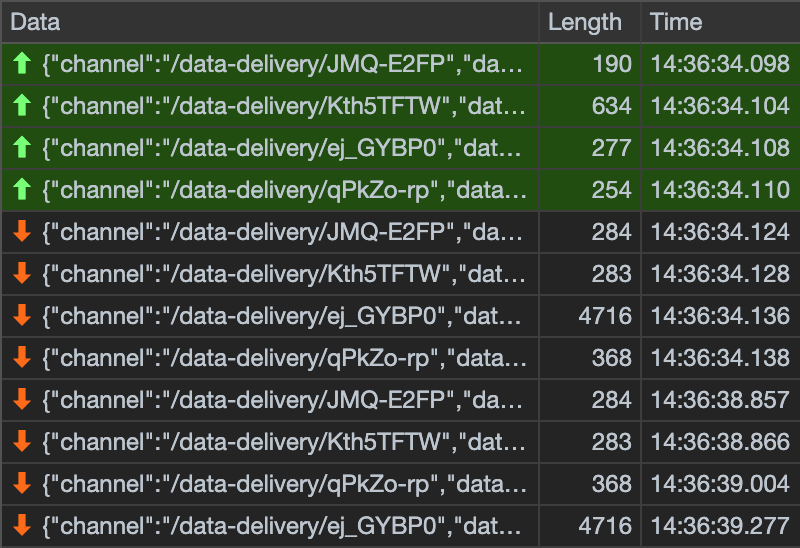
\includegraphics[scale=0.65]{img/screenshots/WebSocketTraffic}
    \end{center}
    \caption{Screenshot des WebSocket-Datenverkehrs}
\end{figure}
% Erkenntnis, Der Cache ist viel schneller, Cache ist O(1) wohingegen datenverarbeitung O(n) ist siehe
% anhand der größeren Anfrage
